\documentclass[twoside]{book}

% Packages required by doxygen
\usepackage{fixltx2e}
\usepackage{calc}
\usepackage{doxygen}
\usepackage[export]{adjustbox} % also loads graphicx
\usepackage{graphicx}
\usepackage[utf8]{inputenc}
\usepackage{makeidx}
\usepackage{multicol}
\usepackage{multirow}
\PassOptionsToPackage{warn}{textcomp}
\usepackage{textcomp}
\usepackage[nointegrals]{wasysym}
\usepackage[table]{xcolor}

% Font selection
\usepackage[T1]{fontenc}
\usepackage[scaled=.90]{helvet}
\usepackage{courier}
\usepackage{amssymb}
\usepackage{sectsty}
\renewcommand{\familydefault}{\sfdefault}
\allsectionsfont{%
  \fontseries{bc}\selectfont%
  \color{darkgray}%
}
\renewcommand{\DoxyLabelFont}{%
  \fontseries{bc}\selectfont%
  \color{darkgray}%
}
\newcommand{\+}{\discretionary{\mbox{\scriptsize$\hookleftarrow$}}{}{}}

% Page & text layout
\usepackage{geometry}
\geometry{%
  a4paper,%
  top=2.5cm,%
  bottom=2.5cm,%
  left=2.5cm,%
  right=2.5cm%
}
\tolerance=750
\hfuzz=15pt
\hbadness=750
\setlength{\emergencystretch}{15pt}
\setlength{\parindent}{0cm}
\setlength{\parskip}{3ex plus 2ex minus 2ex}
\makeatletter
\renewcommand{\paragraph}{%
  \@startsection{paragraph}{4}{0ex}{-1.0ex}{1.0ex}{%
    \normalfont\normalsize\bfseries\SS@parafont%
  }%
}
\renewcommand{\subparagraph}{%
  \@startsection{subparagraph}{5}{0ex}{-1.0ex}{1.0ex}{%
    \normalfont\normalsize\bfseries\SS@subparafont%
  }%
}
\makeatother

% Headers & footers
\usepackage{fancyhdr}
\pagestyle{fancyplain}
\fancyhead[LE]{\fancyplain{}{\bfseries\thepage}}
\fancyhead[CE]{\fancyplain{}{}}
\fancyhead[RE]{\fancyplain{}{\bfseries\leftmark}}
\fancyhead[LO]{\fancyplain{}{\bfseries\rightmark}}
\fancyhead[CO]{\fancyplain{}{}}
\fancyhead[RO]{\fancyplain{}{\bfseries\thepage}}
\fancyfoot[LE]{\fancyplain{}{}}
\fancyfoot[CE]{\fancyplain{}{}}
\fancyfoot[RE]{\fancyplain{}{\bfseries\scriptsize Generated by Doxygen }}
\fancyfoot[LO]{\fancyplain{}{\bfseries\scriptsize Generated by Doxygen }}
\fancyfoot[CO]{\fancyplain{}{}}
\fancyfoot[RO]{\fancyplain{}{}}
\renewcommand{\footrulewidth}{0.4pt}
\renewcommand{\chaptermark}[1]{%
  \markboth{#1}{}%
}
\renewcommand{\sectionmark}[1]{%
  \markright{\thesection\ #1}%
}

% Indices & bibliography
\usepackage{natbib}
\usepackage[titles]{tocloft}
\setcounter{tocdepth}{3}
\setcounter{secnumdepth}{5}
\makeindex

% Hyperlinks (required, but should be loaded last)
\usepackage{ifpdf}
\ifpdf
  \usepackage[pdftex,pagebackref=true]{hyperref}
\else
  \usepackage[ps2pdf,pagebackref=true]{hyperref}
\fi
\hypersetup{%
  colorlinks=true,%
  linkcolor=blue,%
  citecolor=blue,%
  unicode%
}

% Custom commands
\newcommand{\clearemptydoublepage}{%
  \newpage{\pagestyle{empty}\cleardoublepage}%
}

\usepackage{caption}
\captionsetup{labelsep=space,justification=centering,font={bf},singlelinecheck=off,skip=4pt,position=top}

%===== C O N T E N T S =====

\begin{document}

% Titlepage & ToC
\hypersetup{pageanchor=false,
             bookmarksnumbered=true,
             pdfencoding=unicode
            }
\pagenumbering{alph}
\begin{titlepage}
\vspace*{7cm}
\begin{center}%
{\Large Crypto\+Pi }\\
\vspace*{1cm}
{\large Generated by Doxygen 1.8.14}\\
\end{center}
\end{titlepage}
\clearemptydoublepage
\pagenumbering{roman}
\tableofcontents
\clearemptydoublepage
\pagenumbering{arabic}
\hypersetup{pageanchor=true}

%--- Begin generated contents ---
\chapter{Crypto\+Pi -\/ Raspberry Pi web application to monitor changes in crypto-\/currency pairs}
\label{md__r_e_a_d_m_e}
\Hypertarget{md__r_e_a_d_m_e}
\paragraph*{Simply open the app in your browser, input parameters, and monitor!}

\subsection*{Installation instructions\+:}


\begin{DoxyItemize}
\item Clone the repository
\item Compile \href{https://github.com/gurpinars/bittrex-cpp}{\tt Bittrex}
\item Compile \href{https://github.com/MMquant/bfx-cpp-api}{\tt Bitfinex}
\end{DoxyItemize}

(G\+Dax is compiled with the project)


\begin{DoxyItemize}
\item Compile Wt {\ttfamily sudo apt-\/get install witty witty-\/dev witty-\/doc witty-\/dbg witty-\/examples}
\item {\ttfamily make} to build the app
\item {\ttfamily make run} to run
\end{DoxyItemize}

\subsection*{Screenshot\+:}

 
\chapter{Hierarchical Index}
\section{Class Hierarchy}
This inheritance list is sorted roughly, but not completely, alphabetically\+:\begin{DoxyCompactList}
\item \contentsline{section}{Bitfinex\+Trade\+Pair}{\pageref{class_bitfinex_trade_pair}}{}
\item \contentsline{section}{Bittrex\+Trade\+Pair}{\pageref{class_bittrex_trade_pair}}{}
\item \contentsline{section}{client\+\_\+gdax}{\pageref{classclient__gdax}}{}
\item \contentsline{section}{f\+\_\+data}{\pageref{structf__data}}{}
\item \contentsline{section}{Gdax\+Trade\+Pair}{\pageref{class_gdax_trade_pair}}{}
\item \contentsline{section}{mkt\+\_\+symbol}{\pageref{structmkt__symbol}}{}
\item \contentsline{section}{order}{\pageref{structorder}}{}
\item \contentsline{section}{Trade\+Pair}{\pageref{class_trade_pair}}{}
\item W\+Application\begin{DoxyCompactList}
\item \contentsline{section}{Crypto\+Pi\+Main}{\pageref{class_crypto_pi_main}}{}
\end{DoxyCompactList}
\end{DoxyCompactList}

\chapter{Class Index}
\section{Class List}
Here are the classes, structs, unions and interfaces with brief descriptions\+:\begin{DoxyCompactList}
\item\contentsline{section}{\mbox{\hyperlink{class_bitfinex_trade_pair}{Bitfinex\+Trade\+Pair}} }{\pageref{class_bitfinex_trade_pair}}{}
\item\contentsline{section}{\mbox{\hyperlink{class_bittrex_trade_pair}{Bittrex\+Trade\+Pair}} }{\pageref{class_bittrex_trade_pair}}{}
\item\contentsline{section}{\mbox{\hyperlink{classclient__gdax}{client\+\_\+gdax}} }{\pageref{classclient__gdax}}{}
\item\contentsline{section}{\mbox{\hyperlink{class_crypto_pi_main}{Crypto\+Pi\+Main}} }{\pageref{class_crypto_pi_main}}{}
\item\contentsline{section}{\mbox{\hyperlink{structf__data}{f\+\_\+data}} }{\pageref{structf__data}}{}
\item\contentsline{section}{\mbox{\hyperlink{class_gdax_trade_pair}{Gdax\+Trade\+Pair}} }{\pageref{class_gdax_trade_pair}}{}
\item\contentsline{section}{\mbox{\hyperlink{structmkt__symbol}{mkt\+\_\+symbol}} }{\pageref{structmkt__symbol}}{}
\item\contentsline{section}{\mbox{\hyperlink{structorder}{order}} }{\pageref{structorder}}{}
\item\contentsline{section}{\mbox{\hyperlink{class_trade_pair}{Trade\+Pair}} }{\pageref{class_trade_pair}}{}
\end{DoxyCompactList}

\chapter{Class Documentation}
\hypertarget{class_bitfinex_trade_pair}{}\section{Bitfinex\+Trade\+Pair Class Reference}
\label{class_bitfinex_trade_pair}\index{Bitfinex\+Trade\+Pair@{Bitfinex\+Trade\+Pair}}
\subsection*{Public Member Functions}
\begin{DoxyCompactItemize}
\item 
\mbox{\Hypertarget{class_bitfinex_trade_pair_a1d82651543f1facdff8fecb86efdf718}\label{class_bitfinex_trade_pair_a1d82651543f1facdff8fecb86efdf718}} 
\mbox{\hyperlink{class_bitfinex_trade_pair_a1d82651543f1facdff8fecb86efdf718}{Bitfinex\+Trade\+Pair}} (std\+::string name)
\begin{DoxyCompactList}\small\item\em constructor \end{DoxyCompactList}\item 
\mbox{\Hypertarget{class_bitfinex_trade_pair_ad2a01ffb120afa0939d8d41dc6e34686}\label{class_bitfinex_trade_pair_ad2a01ffb120afa0939d8d41dc6e34686}} 
\mbox{\hyperlink{class_bitfinex_trade_pair_ad2a01ffb120afa0939d8d41dc6e34686}{$\sim$\+Bitfinex\+Trade\+Pair}} ()
\begin{DoxyCompactList}\small\item\em destructor \end{DoxyCompactList}\item 
std\+::string \mbox{\hyperlink{class_bitfinex_trade_pair_a2c772425f29358b17e38f2c35fcdb69f}{pair\+Convert}} (std\+::string str)
\item 
std\+::string \mbox{\hyperlink{class_bitfinex_trade_pair_ac00dfde40f1d2a1d00bf8054d442bfac}{get\+Name}} ()
\begin{DoxyCompactList}\small\item\em returns the name \end{DoxyCompactList}\item 
double \mbox{\hyperlink{class_bitfinex_trade_pair_a5e9752e1d32db469a3ce368bc1de2886}{fetch\+Volume}} ()
\item 
double \mbox{\hyperlink{class_bitfinex_trade_pair_ac87f08ef5793dbb17b04798227400aab}{fetch\+Volume\+Change}} ()
\begin{DoxyCompactList}\small\item\em returns the volume change by creating a new volume first \end{DoxyCompactList}\item 
double \mbox{\hyperlink{class_bitfinex_trade_pair_aa0e8da551d808f9d64be6f322120777e}{get\+Volume}} ()
\begin{DoxyCompactList}\small\item\em returns the volume \end{DoxyCompactList}\item 
void \mbox{\hyperlink{class_bitfinex_trade_pair_a0fd67bf84f3221538bbceb434a603f34}{set\+Volume}} (double vol)
\begin{DoxyCompactList}\small\item\em sets the volume \end{DoxyCompactList}\item 
double \mbox{\hyperlink{class_bitfinex_trade_pair_a6ae365c882e5950c87fbfba9058b24ac}{fetch\+Price}} ()
\item 
double \mbox{\hyperlink{class_bitfinex_trade_pair_ac28554bdf8f8397e8d751c792aebf948}{fetch\+Price\+Change}} ()
\begin{DoxyCompactList}\small\item\em returns the price change by creating a new price first \end{DoxyCompactList}\item 
double \mbox{\hyperlink{class_bitfinex_trade_pair_a4dc226e8c0dcadbb0ea39381428721a6}{get\+Price}} ()
\begin{DoxyCompactList}\small\item\em returns the price \end{DoxyCompactList}\item 
void \mbox{\hyperlink{class_bitfinex_trade_pair_ada35f305bafd57ad58cabf20241bec7f}{set\+Price}} (double pri)
\begin{DoxyCompactList}\small\item\em sets the price \end{DoxyCompactList}\end{DoxyCompactItemize}
\subsection*{Friends}
\begin{DoxyCompactItemize}
\item 
\mbox{\Hypertarget{class_bitfinex_trade_pair_aad9f3bb5f4015f3e9b87556ad33f46d7}\label{class_bitfinex_trade_pair_aad9f3bb5f4015f3e9b87556ad33f46d7}} 
std\+::ostream \& \mbox{\hyperlink{class_bitfinex_trade_pair_aad9f3bb5f4015f3e9b87556ad33f46d7}{operator$<$$<$}} (std\+::ostream \&os, const \mbox{\hyperlink{class_bitfinex_trade_pair}{Bitfinex\+Trade\+Pair}} \&vp)
\begin{DoxyCompactList}\small\item\em simple method to return output as ostream \end{DoxyCompactList}\end{DoxyCompactItemize}


\subsection{Member Function Documentation}
\mbox{\Hypertarget{class_bitfinex_trade_pair_a6ae365c882e5950c87fbfba9058b24ac}\label{class_bitfinex_trade_pair_a6ae365c882e5950c87fbfba9058b24ac}} 
\index{Bitfinex\+Trade\+Pair@{Bitfinex\+Trade\+Pair}!fetch\+Price@{fetch\+Price}}
\index{fetch\+Price@{fetch\+Price}!Bitfinex\+Trade\+Pair@{Bitfinex\+Trade\+Pair}}
\subsubsection{\texorpdfstring{fetch\+Price()}{fetchPrice()}}
{\footnotesize\ttfamily double Bitfinex\+Trade\+Pair\+::fetch\+Price (\begin{DoxyParamCaption}{ }\end{DoxyParamCaption})}

this function will get us the price from the bitfinex library this library however return the information as a string which means that we have to use boost and get whatever we went out of that string \mbox{\Hypertarget{class_bitfinex_trade_pair_ac28554bdf8f8397e8d751c792aebf948}\label{class_bitfinex_trade_pair_ac28554bdf8f8397e8d751c792aebf948}} 
\index{Bitfinex\+Trade\+Pair@{Bitfinex\+Trade\+Pair}!fetch\+Price\+Change@{fetch\+Price\+Change}}
\index{fetch\+Price\+Change@{fetch\+Price\+Change}!Bitfinex\+Trade\+Pair@{Bitfinex\+Trade\+Pair}}
\subsubsection{\texorpdfstring{fetch\+Price\+Change()}{fetchPriceChange()}}
{\footnotesize\ttfamily double Bitfinex\+Trade\+Pair\+::fetch\+Price\+Change (\begin{DoxyParamCaption}{ }\end{DoxyParamCaption})}



returns the price change by creating a new price first 

this function will get a new price and then divide our old price by the new price to get price change \mbox{\Hypertarget{class_bitfinex_trade_pair_a5e9752e1d32db469a3ce368bc1de2886}\label{class_bitfinex_trade_pair_a5e9752e1d32db469a3ce368bc1de2886}} 
\index{Bitfinex\+Trade\+Pair@{Bitfinex\+Trade\+Pair}!fetch\+Volume@{fetch\+Volume}}
\index{fetch\+Volume@{fetch\+Volume}!Bitfinex\+Trade\+Pair@{Bitfinex\+Trade\+Pair}}
\subsubsection{\texorpdfstring{fetch\+Volume()}{fetchVolume()}}
{\footnotesize\ttfamily double Bitfinex\+Trade\+Pair\+::fetch\+Volume (\begin{DoxyParamCaption}{ }\end{DoxyParamCaption})}

this function will get us the volume from the bitfinex library this library however return the information as a string which means that we have to use boost and get whatever we went out of that string \mbox{\Hypertarget{class_bitfinex_trade_pair_ac87f08ef5793dbb17b04798227400aab}\label{class_bitfinex_trade_pair_ac87f08ef5793dbb17b04798227400aab}} 
\index{Bitfinex\+Trade\+Pair@{Bitfinex\+Trade\+Pair}!fetch\+Volume\+Change@{fetch\+Volume\+Change}}
\index{fetch\+Volume\+Change@{fetch\+Volume\+Change}!Bitfinex\+Trade\+Pair@{Bitfinex\+Trade\+Pair}}
\subsubsection{\texorpdfstring{fetch\+Volume\+Change()}{fetchVolumeChange()}}
{\footnotesize\ttfamily double Bitfinex\+Trade\+Pair\+::fetch\+Volume\+Change (\begin{DoxyParamCaption}{ }\end{DoxyParamCaption})}



returns the volume change by creating a new volume first 

this function will return the volume change by geting a new volume and dividing it by old volume \mbox{\Hypertarget{class_bitfinex_trade_pair_ac00dfde40f1d2a1d00bf8054d442bfac}\label{class_bitfinex_trade_pair_ac00dfde40f1d2a1d00bf8054d442bfac}} 
\index{Bitfinex\+Trade\+Pair@{Bitfinex\+Trade\+Pair}!get\+Name@{get\+Name}}
\index{get\+Name@{get\+Name}!Bitfinex\+Trade\+Pair@{Bitfinex\+Trade\+Pair}}
\subsubsection{\texorpdfstring{get\+Name()}{getName()}}
{\footnotesize\ttfamily std\+::string Bitfinex\+Trade\+Pair\+::get\+Name (\begin{DoxyParamCaption}{ }\end{DoxyParamCaption})}



returns the name 

this function returns the name of the trade pair \mbox{\Hypertarget{class_bitfinex_trade_pair_a4dc226e8c0dcadbb0ea39381428721a6}\label{class_bitfinex_trade_pair_a4dc226e8c0dcadbb0ea39381428721a6}} 
\index{Bitfinex\+Trade\+Pair@{Bitfinex\+Trade\+Pair}!get\+Price@{get\+Price}}
\index{get\+Price@{get\+Price}!Bitfinex\+Trade\+Pair@{Bitfinex\+Trade\+Pair}}
\subsubsection{\texorpdfstring{get\+Price()}{getPrice()}}
{\footnotesize\ttfamily double Bitfinex\+Trade\+Pair\+::get\+Price (\begin{DoxyParamCaption}{ }\end{DoxyParamCaption})}



returns the price 

returns price \mbox{\Hypertarget{class_bitfinex_trade_pair_aa0e8da551d808f9d64be6f322120777e}\label{class_bitfinex_trade_pair_aa0e8da551d808f9d64be6f322120777e}} 
\index{Bitfinex\+Trade\+Pair@{Bitfinex\+Trade\+Pair}!get\+Volume@{get\+Volume}}
\index{get\+Volume@{get\+Volume}!Bitfinex\+Trade\+Pair@{Bitfinex\+Trade\+Pair}}
\subsubsection{\texorpdfstring{get\+Volume()}{getVolume()}}
{\footnotesize\ttfamily double Bitfinex\+Trade\+Pair\+::get\+Volume (\begin{DoxyParamCaption}{ }\end{DoxyParamCaption})}



returns the volume 

this function returns the volume of the trade pair \mbox{\Hypertarget{class_bitfinex_trade_pair_a2c772425f29358b17e38f2c35fcdb69f}\label{class_bitfinex_trade_pair_a2c772425f29358b17e38f2c35fcdb69f}} 
\index{Bitfinex\+Trade\+Pair@{Bitfinex\+Trade\+Pair}!pair\+Convert@{pair\+Convert}}
\index{pair\+Convert@{pair\+Convert}!Bitfinex\+Trade\+Pair@{Bitfinex\+Trade\+Pair}}
\subsubsection{\texorpdfstring{pair\+Convert()}{pairConvert()}}
{\footnotesize\ttfamily std\+::string Bitfinex\+Trade\+Pair\+::pair\+Convert (\begin{DoxyParamCaption}\item[{std\+::string}]{str }\end{DoxyParamCaption})}

this function will change the input into an acceptable input for bitfinex since bitfinux only accepts input as \char`\"{}btcusd\char`\"{} type and we only use \char`\"{}\+B\+T\+C-\/\+U\+S\+D\char`\"{} we need to change the input for bitfiniex to retrieve the information \mbox{\Hypertarget{class_bitfinex_trade_pair_ada35f305bafd57ad58cabf20241bec7f}\label{class_bitfinex_trade_pair_ada35f305bafd57ad58cabf20241bec7f}} 
\index{Bitfinex\+Trade\+Pair@{Bitfinex\+Trade\+Pair}!set\+Price@{set\+Price}}
\index{set\+Price@{set\+Price}!Bitfinex\+Trade\+Pair@{Bitfinex\+Trade\+Pair}}
\subsubsection{\texorpdfstring{set\+Price()}{setPrice()}}
{\footnotesize\ttfamily void Bitfinex\+Trade\+Pair\+::set\+Price (\begin{DoxyParamCaption}\item[{double}]{pri }\end{DoxyParamCaption})}



sets the price 

sets price \mbox{\Hypertarget{class_bitfinex_trade_pair_a0fd67bf84f3221538bbceb434a603f34}\label{class_bitfinex_trade_pair_a0fd67bf84f3221538bbceb434a603f34}} 
\index{Bitfinex\+Trade\+Pair@{Bitfinex\+Trade\+Pair}!set\+Volume@{set\+Volume}}
\index{set\+Volume@{set\+Volume}!Bitfinex\+Trade\+Pair@{Bitfinex\+Trade\+Pair}}
\subsubsection{\texorpdfstring{set\+Volume()}{setVolume()}}
{\footnotesize\ttfamily void Bitfinex\+Trade\+Pair\+::set\+Volume (\begin{DoxyParamCaption}\item[{double}]{vol }\end{DoxyParamCaption})}



sets the volume 

this function sets the volume of the trade pair 

The documentation for this class was generated from the following files\+:\begin{DoxyCompactItemize}
\item 
Bitfinex\+Trade\+Pair.\+h\item 
Bitfinex\+Trade\+Pair.\+cpp\end{DoxyCompactItemize}

\hypertarget{class_bittrex_trade_pair}{}\section{Bittrex\+Trade\+Pair Class Reference}
\label{class_bittrex_trade_pair}\index{Bittrex\+Trade\+Pair@{Bittrex\+Trade\+Pair}}
\subsection*{Public Member Functions}
\begin{DoxyCompactItemize}
\item 
\mbox{\Hypertarget{class_bittrex_trade_pair_ab6da87febee0387eb320553ccd0dc4ce}\label{class_bittrex_trade_pair_ab6da87febee0387eb320553ccd0dc4ce}} 
\mbox{\hyperlink{class_bittrex_trade_pair_ab6da87febee0387eb320553ccd0dc4ce}{Bittrex\+Trade\+Pair}} (std\+::string name)
\begin{DoxyCompactList}\small\item\em constructor \end{DoxyCompactList}\item 
\mbox{\Hypertarget{class_bittrex_trade_pair_a13b7e834b50ce3b7f773a40d7a4828a6}\label{class_bittrex_trade_pair_a13b7e834b50ce3b7f773a40d7a4828a6}} 
\mbox{\hyperlink{class_bittrex_trade_pair_a13b7e834b50ce3b7f773a40d7a4828a6}{$\sim$\+Bittrex\+Trade\+Pair}} ()
\begin{DoxyCompactList}\small\item\em destructor \end{DoxyCompactList}\item 
\mbox{\Hypertarget{class_bittrex_trade_pair_aabb1730857c694a64b15eaf5824ec72a}\label{class_bittrex_trade_pair_aabb1730857c694a64b15eaf5824ec72a}} 
std\+::string \mbox{\hyperlink{class_bittrex_trade_pair_aabb1730857c694a64b15eaf5824ec72a}{get\+Name}} ()
\begin{DoxyCompactList}\small\item\em getters and setters \end{DoxyCompactList}\item 
double \mbox{\hyperlink{class_bittrex_trade_pair_a314efdd2917c88f48cd521dacf4eed85}{fetch\+Volume}} ()
\begin{DoxyCompactList}\small\item\em to grab the volume for a specific pair passed in by the front end \end{DoxyCompactList}\item 
\mbox{\Hypertarget{class_bittrex_trade_pair_afd555c5ae36025d25964350c50f1006a}\label{class_bittrex_trade_pair_afd555c5ae36025d25964350c50f1006a}} 
double \mbox{\hyperlink{class_bittrex_trade_pair_afd555c5ae36025d25964350c50f1006a}{fetch\+Volume\+Change}} ()
\begin{DoxyCompactList}\small\item\em creates new volume then compares to old volume to get volume change \end{DoxyCompactList}\item 
\mbox{\Hypertarget{class_bittrex_trade_pair_ac3e959d5d6aa90c9126e8f31c1b8d6f8}\label{class_bittrex_trade_pair_ac3e959d5d6aa90c9126e8f31c1b8d6f8}} 
double {\bfseries get\+Volume} ()
\item 
\mbox{\Hypertarget{class_bittrex_trade_pair_a40f9c9ff6618e1a170820bd60daeaa0f}\label{class_bittrex_trade_pair_a40f9c9ff6618e1a170820bd60daeaa0f}} 
void {\bfseries set\+Volume} (double vol)
\item 
double \mbox{\hyperlink{class_bittrex_trade_pair_a74564273a0a56f63a8737fbb4b0dc2e5}{fetch\+Price}} ()
\begin{DoxyCompactList}\small\item\em to grab the volume for a specific pair passed in by the front end \end{DoxyCompactList}\item 
\mbox{\Hypertarget{class_bittrex_trade_pair_add7f130337294db2b56ce2fbcc669c90}\label{class_bittrex_trade_pair_add7f130337294db2b56ce2fbcc669c90}} 
double \mbox{\hyperlink{class_bittrex_trade_pair_add7f130337294db2b56ce2fbcc669c90}{fetch\+Price\+Change}} ()
\begin{DoxyCompactList}\small\item\em creates a new price then compares to old price to get price change \end{DoxyCompactList}\item 
\mbox{\Hypertarget{class_bittrex_trade_pair_af0a18d8b1cc841b657a474ea071e9778}\label{class_bittrex_trade_pair_af0a18d8b1cc841b657a474ea071e9778}} 
double {\bfseries get\+Price} ()
\item 
\mbox{\Hypertarget{class_bittrex_trade_pair_a59673b3475518b65d45651b2a1b0f581}\label{class_bittrex_trade_pair_a59673b3475518b65d45651b2a1b0f581}} 
void {\bfseries set\+Price} (double pri)
\end{DoxyCompactItemize}
\subsection*{Friends}
\begin{DoxyCompactItemize}
\item 
\mbox{\Hypertarget{class_bittrex_trade_pair_a1fc3a2979f802733275f0d907c8ddcb6}\label{class_bittrex_trade_pair_a1fc3a2979f802733275f0d907c8ddcb6}} 
std\+::ostream \& \mbox{\hyperlink{class_bittrex_trade_pair_a1fc3a2979f802733275f0d907c8ddcb6}{operator$<$$<$}} (std\+::ostream \&os, const \mbox{\hyperlink{class_bittrex_trade_pair}{Bittrex\+Trade\+Pair}} \&vp)
\begin{DoxyCompactList}\small\item\em returns our price and volume as an ostream \end{DoxyCompactList}\end{DoxyCompactItemize}


\subsection{Member Function Documentation}
\mbox{\Hypertarget{class_bittrex_trade_pair_a74564273a0a56f63a8737fbb4b0dc2e5}\label{class_bittrex_trade_pair_a74564273a0a56f63a8737fbb4b0dc2e5}} 
\index{Bittrex\+Trade\+Pair@{Bittrex\+Trade\+Pair}!fetch\+Price@{fetch\+Price}}
\index{fetch\+Price@{fetch\+Price}!Bittrex\+Trade\+Pair@{Bittrex\+Trade\+Pair}}
\subsubsection{\texorpdfstring{fetch\+Price()}{fetchPrice()}}
{\footnotesize\ttfamily double Bittrex\+Trade\+Pair\+::fetch\+Price (\begin{DoxyParamCaption}{ }\end{DoxyParamCaption})}



to grab the volume for a specific pair passed in by the front end 

this function gets the price from the public library the key and secret are not used but needed to compile the code we dont use them because we dont need identification since we are not trading summary creates the object of type summary and then vol gets exactly what we want from that summary then returns it \mbox{\Hypertarget{class_bittrex_trade_pair_a314efdd2917c88f48cd521dacf4eed85}\label{class_bittrex_trade_pair_a314efdd2917c88f48cd521dacf4eed85}} 
\index{Bittrex\+Trade\+Pair@{Bittrex\+Trade\+Pair}!fetch\+Volume@{fetch\+Volume}}
\index{fetch\+Volume@{fetch\+Volume}!Bittrex\+Trade\+Pair@{Bittrex\+Trade\+Pair}}
\subsubsection{\texorpdfstring{fetch\+Volume()}{fetchVolume()}}
{\footnotesize\ttfamily double Bittrex\+Trade\+Pair\+::fetch\+Volume (\begin{DoxyParamCaption}{ }\end{DoxyParamCaption})}



to grab the volume for a specific pair passed in by the front end 

this function gets the volume from the public library the key and secret are not used but needed to compile the code we dont use them because we dont need identification since we are not trading summary creates the object of type summary and then vol gets exactly what we want from that summary then returns it 

The documentation for this class was generated from the following files\+:\begin{DoxyCompactItemize}
\item 
Bittrex\+Trade\+Pair.\+h\item 
Bittrex\+Trade\+Pair.\+cpp\end{DoxyCompactItemize}

\hypertarget{classclient__gdax}{}\section{client\+\_\+gdax Class Reference}
\label{classclient__gdax}\index{client\+\_\+gdax@{client\+\_\+gdax}}
\subsection*{Public Member Functions}
\begin{DoxyCompactItemize}
\item 
\mbox{\Hypertarget{classclient__gdax_a1e4d7c2f08a89acabecc0a7ac1e2ae50}\label{classclient__gdax_a1e4d7c2f08a89acabecc0a7ac1e2ae50}} 
{\bfseries client\+\_\+gdax} (std\+::string key, std\+::string secret, std\+::string passphrase)
\item 
\mbox{\Hypertarget{classclient__gdax_a202eea2735b0d2c98c859e2bd9e6e584}\label{classclient__gdax_a202eea2735b0d2c98c859e2bd9e6e584}} 
std\+::string {\bfseries sign\+\_\+data} (const char $\ast$data, std\+::size\+\_\+t data\+\_\+size, std\+::string my\+\_\+key)
\item 
\mbox{\Hypertarget{classclient__gdax_aac03123e9a85dd08d56ffb94e0f90811}\label{classclient__gdax_aac03123e9a85dd08d56ffb94e0f90811}} 
std\+::string {\bfseries return\+Trade\+History} (\mbox{\hyperlink{structmkt__symbol}{mkt\+\_\+symbol}} currency\+Pair)
\item 
\mbox{\Hypertarget{classclient__gdax_a584e3c9f8da2dd4c90c7111bc9d88e17}\label{classclient__gdax_a584e3c9f8da2dd4c90c7111bc9d88e17}} 
std\+::string {\bfseries return\+Available\+Account\+Balances} ()
\item 
\mbox{\Hypertarget{classclient__gdax_a8983b5020b86571b40e1165facab03cd}\label{classclient__gdax_a8983b5020b86571b40e1165facab03cd}} 
int {\bfseries return\+Order\+Trades\+\_\+vec} (\mbox{\hyperlink{structorder}{order}} \&o1, std\+::string \&err\+\_\+str, std\+::string input\+\_\+str=\char`\"{}-\/99\char`\"{})
\item 
\mbox{\Hypertarget{classclient__gdax_a0e1fe01089c66788d95db9bda0d6fde4}\label{classclient__gdax_a0e1fe01089c66788d95db9bda0d6fde4}} 
std\+::string {\bfseries move} (\mbox{\hyperlink{structorder}{order}} \&o1, double price, double amount=0)
\item 
\mbox{\Hypertarget{classclient__gdax_a59642a0c813e5c25e103e6b9c0c4402d}\label{classclient__gdax_a59642a0c813e5c25e103e6b9c0c4402d}} 
int {\bfseries move\+\_\+vec} (\mbox{\hyperlink{structorder}{order}} \&o1, \mbox{\hyperlink{structorder}{order}} \&new\+\_\+order, double price, std\+::string \&err\+\_\+str, double amount=-\/99, std\+::string input\+\_\+str=\char`\"{}-\/99\char`\"{})
\item 
\mbox{\Hypertarget{classclient__gdax_aa0476039a3b2f149452aecae545174f1}\label{classclient__gdax_aa0476039a3b2f149452aecae545174f1}} 
int {\bfseries get\+Base64} (const std\+::string \&content, std\+::string \&encoded)
\item 
\mbox{\Hypertarget{classclient__gdax_a0bc53d1588520768f5e63ecf93b66c78}\label{classclient__gdax_a0bc53d1588520768f5e63ecf93b66c78}} 
std\+::string {\bfseries return\+Open\+Orders} (std\+::string str1)
\item 
\mbox{\Hypertarget{classclient__gdax_a9395e877baf8c69343e9b9e6792bc403}\label{classclient__gdax_a9395e877baf8c69343e9b9e6792bc403}} 
int {\bfseries Dorequest} (const std\+::string \&Url\+End\+Point, const std\+::string \&body, std\+::string \&result, const std\+::string \&method, const std\+::string \&request\+\_\+path)
\item 
\mbox{\Hypertarget{classclient__gdax_a2ae55cb58430803493b370cf73fb8089}\label{classclient__gdax_a2ae55cb58430803493b370cf73fb8089}} 
std\+::string {\bfseries make\+\_\+gdax\+\_\+sym} (\mbox{\hyperlink{structmkt__symbol}{mkt\+\_\+symbol}} m)
\item 
\mbox{\Hypertarget{classclient__gdax_a0f3e334bbaebc75cf56f27cf7783f999}\label{classclient__gdax_a0f3e334bbaebc75cf56f27cf7783f999}} 
int {\bfseries Decode\+Base64} (const std\+::string \&encoded, std\+::string \&decoded)
\item 
\mbox{\Hypertarget{classclient__gdax_a37776491211b838c1ad158a175080020}\label{classclient__gdax_a37776491211b838c1ad158a175080020}} 
int {\bfseries get\+Hmac\+Sha256} (const std\+::string \&key, const std\+::string \&content, std\+::string \&digest)
\item 
\mbox{\Hypertarget{classclient__gdax_aef2b4a68ce70c604a29c57496f129741}\label{classclient__gdax_aef2b4a68ce70c604a29c57496f129741}} 
std\+::string {\bfseries cancel\+Order} (std\+::string ordernum)
\item 
\mbox{\Hypertarget{classclient__gdax_ac15410e231beae59a576d82095ddfe71}\label{classclient__gdax_ac15410e231beae59a576d82095ddfe71}} 
std\+::string {\bfseries Generate\+Check\+Sum} (const char $\ast$buf, long buf\+Len)
\item 
\mbox{\Hypertarget{classclient__gdax_adf9a3134a5e5835a1a2993889253cece}\label{classclient__gdax_adf9a3134a5e5835a1a2993889253cece}} 
std\+::string {\bfseries gettime} ()
\item 
\mbox{\Hypertarget{classclient__gdax_a27e0b53b9b8a18b6c898f2ae09d1c383}\label{classclient__gdax_a27e0b53b9b8a18b6c898f2ae09d1c383}} 
std\+::string {\bfseries make\+\_\+fix} (std\+::vector$<$ \mbox{\hyperlink{structf__data}{f\+\_\+data}} $>$ x)
\item 
\mbox{\Hypertarget{classclient__gdax_ac99bed19bf6b219dddb3f8b53d4a87ac}\label{classclient__gdax_ac99bed19bf6b219dddb3f8b53d4a87ac}} 
const std\+::vector$<$ uint8\+\_\+t $>$ {\bfseries sha256} (const std\+::vector$<$ uint8\+\_\+t $>$ \&key, const std\+::vector$<$ uint8\+\_\+t $>$ \&value)
\item 
\mbox{\Hypertarget{classclient__gdax_af3ecf2ad12ca9855a4f076c81c37c7fe}\label{classclient__gdax_af3ecf2ad12ca9855a4f076c81c37c7fe}} 
std\+::string {\bfseries return\+Order\+Trades} (std\+::string ordernum)
\item 
\mbox{\Hypertarget{classclient__gdax_a23b8769e187a810399bb856633e9c8bc}\label{classclient__gdax_a23b8769e187a810399bb856633e9c8bc}} 
int {\bfseries place\+\_\+order} (\mbox{\hyperlink{structmkt__symbol}{mkt\+\_\+symbol}} symbol, bool isbuy, double price, double quant, \mbox{\hyperlink{structorder}{order}} \&o1, std\+::string \&errstr, std\+::string type\+\_\+order=\char`\"{}exchange limit\char`\"{}, std\+::string input\+\_\+string=\char`\"{}-\/99\char`\"{})
\item 
\mbox{\Hypertarget{classclient__gdax_a7caed201b1416de52ccaeab55ab3f6e2}\label{classclient__gdax_a7caed201b1416de52ccaeab55ab3f6e2}} 
std\+::string {\bfseries get\+\_\+book\+\_\+info} (\mbox{\hyperlink{structmkt__symbol}{mkt\+\_\+symbol}} symbol, int level)
\item 
\mbox{\Hypertarget{classclient__gdax_a314ec11641d65d5a527f181103d65f44}\label{classclient__gdax_a314ec11641d65d5a527f181103d65f44}} 
double {\bfseries get\+\_\+volume\+\_\+info} (std\+::string x)
\item 
\mbox{\Hypertarget{classclient__gdax_a7f2155ab8f30e4cb0c15becc689bc78f}\label{classclient__gdax_a7f2155ab8f30e4cb0c15becc689bc78f}} 
double {\bfseries get\+\_\+price\+\_\+info} (std\+::string x)
\item 
\mbox{\Hypertarget{classclient__gdax_af4d5e2613843e2e2cd074620209389e9}\label{classclient__gdax_af4d5e2613843e2e2cd074620209389e9}} 
int {\bfseries do\+\_\+public\+\_\+request} (const std\+::string \&Url\+End\+Point, std\+::string \&result, const std\+::string \&request\+\_\+path)
\end{DoxyCompactItemize}
\subsection*{Static Public Member Functions}
\begin{DoxyCompactItemize}
\item 
static size\+\_\+t \mbox{\hyperlink{classclient__gdax_aa0cc262133e3443dcf8c0fcbd87a2310}{Write\+Callback}} (void $\ast$contents, size\+\_\+t size, size\+\_\+t nmemb, void $\ast$userp)
\end{DoxyCompactItemize}
\subsection*{Public Attributes}
\begin{DoxyCompactItemize}
\item 
\mbox{\Hypertarget{classclient__gdax_a60857594693d3a1981e4ce15cefed569}\label{classclient__gdax_a60857594693d3a1981e4ce15cefed569}} 
std\+::string {\bfseries A\+P\+Iurl}
\item 
\mbox{\Hypertarget{classclient__gdax_af601c54ba12e81a658e6c1ba4b372ce5}\label{classclient__gdax_af601c54ba12e81a658e6c1ba4b372ce5}} 
std\+::string {\bfseries key}
\item 
\mbox{\Hypertarget{classclient__gdax_a30b02f0cf95ccec98ec21c559121a75d}\label{classclient__gdax_a30b02f0cf95ccec98ec21c559121a75d}} 
std\+::string {\bfseries secret}
\item 
\mbox{\Hypertarget{classclient__gdax_ae8e3321863bea122cb084a9f7ee73521}\label{classclient__gdax_ae8e3321863bea122cb084a9f7ee73521}} 
std\+::string {\bfseries passphrase}
\item 
\mbox{\Hypertarget{classclient__gdax_a6e34720dadbd37c9345eabb1a6496992}\label{classclient__gdax_a6e34720dadbd37c9345eabb1a6496992}} 
C\+U\+RL $\ast$ {\bfseries curl}
\item 
\mbox{\Hypertarget{classclient__gdax_a1bde11c3d715935718e0c96cf5a440eb}\label{classclient__gdax_a1bde11c3d715935718e0c96cf5a440eb}} 
C\+U\+R\+Lcode {\bfseries res}
\item 
\mbox{\Hypertarget{classclient__gdax_accc59af2c0246dbe6bfbba3df019de64}\label{classclient__gdax_accc59af2c0246dbe6bfbba3df019de64}} 
std\+::map$<$ \mbox{\hyperlink{structmkt__symbol}{mkt\+\_\+symbol}}, std\+::string $>$ {\bfseries trade\+\_\+hist\+\_\+pagination}
\item 
\mbox{\Hypertarget{classclient__gdax_ae6071ed094235716d66c8f73d8af75e1}\label{classclient__gdax_ae6071ed094235716d66c8f73d8af75e1}} 
std\+::string {\bfseries fills\+\_\+last\+\_\+id}
\item 
\mbox{\Hypertarget{classclient__gdax_a1d081b59e6acf48a7ffda9fccdb8c5cc}\label{classclient__gdax_a1d081b59e6acf48a7ffda9fccdb8c5cc}} 
bool {\bfseries use\+\_\+\+R\+E\+ST}
\end{DoxyCompactItemize}


\subsection{Member Function Documentation}
\mbox{\Hypertarget{classclient__gdax_aa0cc262133e3443dcf8c0fcbd87a2310}\label{classclient__gdax_aa0cc262133e3443dcf8c0fcbd87a2310}} 
\index{client\+\_\+gdax@{client\+\_\+gdax}!Write\+Callback@{Write\+Callback}}
\index{Write\+Callback@{Write\+Callback}!client\+\_\+gdax@{client\+\_\+gdax}}
\subsubsection{\texorpdfstring{Write\+Callback()}{WriteCallback()}}
{\footnotesize\ttfamily In this case $\ast$userp will point to result size\+\_\+t client\+\_\+gdax\+::\+Write\+Callback (\begin{DoxyParamCaption}\item[{void $\ast$}]{contents,  }\item[{size\+\_\+t}]{size,  }\item[{size\+\_\+t}]{nmemb,  }\item[{void $\ast$}]{userp }\end{DoxyParamCaption})\hspace{0.3cm}{\ttfamily [static]}}

Curl write callback function. Appends fetched $\ast$content to $\ast$userp pointer. / $\ast$userp pointer is set up by curl\+\_\+easy\+\_\+setopt(curl, C\+U\+R\+L\+O\+P\+T\+\_\+\+W\+R\+I\+T\+E\+D\+A\+T\+A, \&result) line. 

The documentation for this class was generated from the following files\+:\begin{DoxyCompactItemize}
\item 
client\+\_\+gdax.\+h\item 
client\+\_\+gdax.\+cpp\end{DoxyCompactItemize}

\hypertarget{class_crypto_pi_main}{}\section{Crypto\+Pi\+Main Class Reference}
\label{class_crypto_pi_main}\index{Crypto\+Pi\+Main@{Crypto\+Pi\+Main}}
Inheritance diagram for Crypto\+Pi\+Main\+:\begin{figure}[H]
\begin{center}
\leavevmode
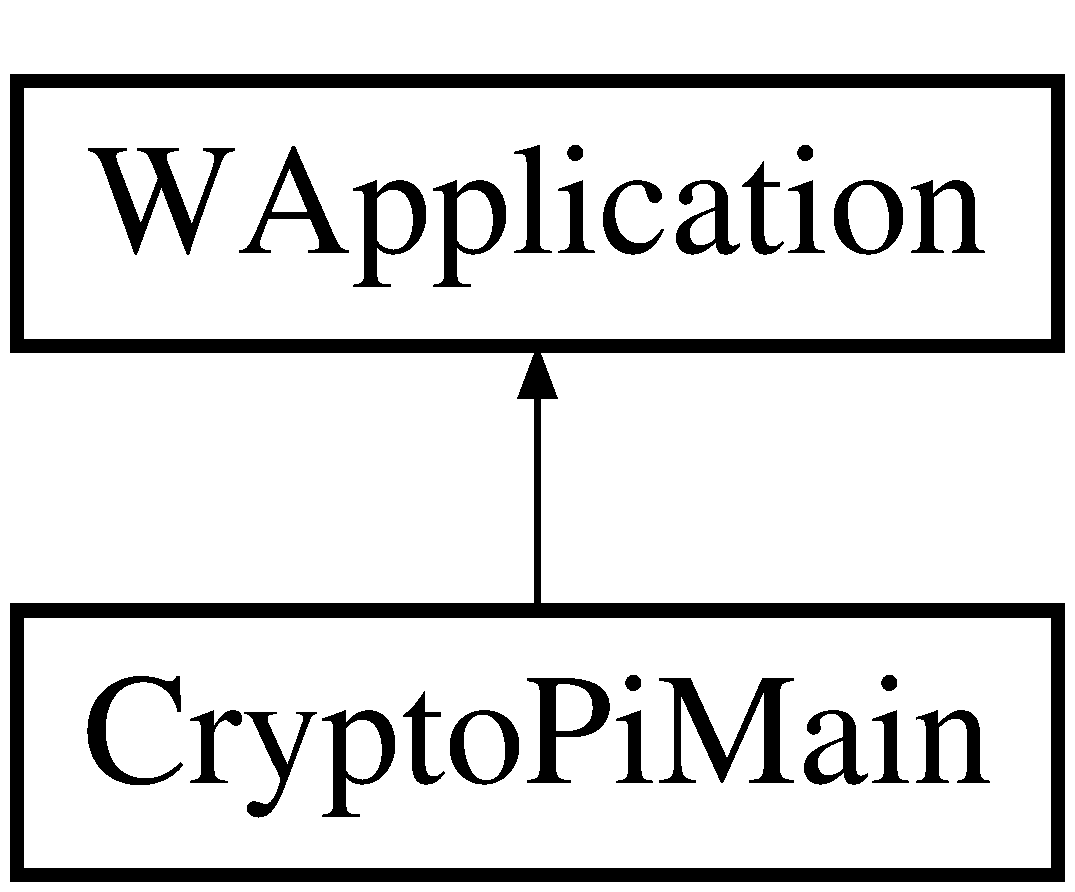
\includegraphics[height=2.000000cm]{class_crypto_pi_main}
\end{center}
\end{figure}
\subsection*{Public Member Functions}
\begin{DoxyCompactItemize}
\item 
\mbox{\Hypertarget{class_crypto_pi_main_ae9442747c64ce69b2369676ec2c86b9b}\label{class_crypto_pi_main_ae9442747c64ce69b2369676ec2c86b9b}} 
{\bfseries Crypto\+Pi\+Main} (const W\+Environment \&env)
\item 
\mbox{\Hypertarget{class_crypto_pi_main_af6ca0336b4524e3452ffcd5780c9b565}\label{class_crypto_pi_main_af6ca0336b4524e3452ffcd5780c9b565}} 
void {\bfseries add\+To\+Monitor} ()
\item 
\mbox{\Hypertarget{class_crypto_pi_main_ad643e4cae4cd1d700f608bf88c9fd510}\label{class_crypto_pi_main_ad643e4cae4cd1d700f608bf88c9fd510}} 
void {\bfseries update\+Table} ()
\item 
\mbox{\Hypertarget{class_crypto_pi_main_acf1d22cffa5010a1010264e6ba2ad1a3}\label{class_crypto_pi_main_acf1d22cffa5010a1010264e6ba2ad1a3}} 
void {\bfseries reset\+Table} ()
\item 
\mbox{\Hypertarget{class_crypto_pi_main_ab6c8cbfd39ee446905e4c7ed8f5b6d98}\label{class_crypto_pi_main_ab6c8cbfd39ee446905e4c7ed8f5b6d98}} 
void {\bfseries update\+Pairs} ()
\end{DoxyCompactItemize}


The documentation for this class was generated from the following file\+:\begin{DoxyCompactItemize}
\item 
main.\+cpp\end{DoxyCompactItemize}

\hypertarget{structf__data}{}\section{f\+\_\+data Struct Reference}
\label{structf__data}\index{f\+\_\+data@{f\+\_\+data}}
\subsection*{Public Member Functions}
\begin{DoxyCompactItemize}
\item 
\mbox{\Hypertarget{structf__data_a1d9dd171db66371468e372138cf72c69}\label{structf__data_a1d9dd171db66371468e372138cf72c69}} 
{\bfseries f\+\_\+data} (int n1, std\+::string message1)
\end{DoxyCompactItemize}
\subsection*{Public Attributes}
\begin{DoxyCompactItemize}
\item 
\mbox{\Hypertarget{structf__data_afdbfdcb60a1554ad6eec9053f575c603}\label{structf__data_afdbfdcb60a1554ad6eec9053f575c603}} 
int {\bfseries n}
\item 
\mbox{\Hypertarget{structf__data_a6783111765c49ed9282dfcb1ce45abd0}\label{structf__data_a6783111765c49ed9282dfcb1ce45abd0}} 
std\+::string {\bfseries message}
\end{DoxyCompactItemize}


The documentation for this struct was generated from the following file\+:\begin{DoxyCompactItemize}
\item 
client\+\_\+gdax.\+h\end{DoxyCompactItemize}

\hypertarget{class_gdax_trade_pair}{}\section{Gdax\+Trade\+Pair Class Reference}
\label{class_gdax_trade_pair}\index{Gdax\+Trade\+Pair@{Gdax\+Trade\+Pair}}
\subsection*{Public Member Functions}
\begin{DoxyCompactItemize}
\item 
\mbox{\Hypertarget{class_gdax_trade_pair_acf77c357616ceb25a568f6dc8196aee5}\label{class_gdax_trade_pair_acf77c357616ceb25a568f6dc8196aee5}} 
\mbox{\hyperlink{class_gdax_trade_pair_acf77c357616ceb25a568f6dc8196aee5}{Gdax\+Trade\+Pair}} (std\+::string name)
\begin{DoxyCompactList}\small\item\em constructor \end{DoxyCompactList}\item 
\mbox{\Hypertarget{class_gdax_trade_pair_a72fe524fa389f64179a595e9e90fc5fc}\label{class_gdax_trade_pair_a72fe524fa389f64179a595e9e90fc5fc}} 
\mbox{\hyperlink{class_gdax_trade_pair_a72fe524fa389f64179a595e9e90fc5fc}{$\sim$\+Gdax\+Trade\+Pair}} ()
\begin{DoxyCompactList}\small\item\em destructor \end{DoxyCompactList}\item 
std\+::string \mbox{\hyperlink{class_gdax_trade_pair_ac67b487345149920a4631b3b2517033f}{get\+Name}} ()
\begin{DoxyCompactList}\small\item\em returns the price pair name \end{DoxyCompactList}\item 
double \mbox{\hyperlink{class_gdax_trade_pair_ad7799585f8c7e06792da997cc53966b5}{fetch\+Volume}} ()
\item 
double \mbox{\hyperlink{class_gdax_trade_pair_ab4bc3b56207898507dd1ea0b2a4d3954}{fetch\+Volume\+Change}} ()
\begin{DoxyCompactList}\small\item\em returns the volume change \end{DoxyCompactList}\item 
double \mbox{\hyperlink{class_gdax_trade_pair_ac1690b5bfce51854585ea1c9288250e6}{get\+Volume}} ()
\begin{DoxyCompactList}\small\item\em returns the volume \end{DoxyCompactList}\item 
void \mbox{\hyperlink{class_gdax_trade_pair_ac9fb00c66634690b9fbb5f2f4a457820}{set\+Volume}} (double vol)
\begin{DoxyCompactList}\small\item\em sets the volume \end{DoxyCompactList}\item 
double \mbox{\hyperlink{class_gdax_trade_pair_adacd391af9a85002ae707c374a1ad17c}{fetch\+Price}} ()
\begin{DoxyCompactList}\small\item\em very similar to the fetch volume except it gets the price \end{DoxyCompactList}\item 
double \mbox{\hyperlink{class_gdax_trade_pair_af6c2de9262607777c2fc22d25b700fc6}{fetch\+Price\+Change}} ()
\begin{DoxyCompactList}\small\item\em returns the price change \end{DoxyCompactList}\item 
double \mbox{\hyperlink{class_gdax_trade_pair_aaec623f9a4d7cb24ee924aa999bfc94a}{get\+Price}} ()
\begin{DoxyCompactList}\small\item\em returns price \end{DoxyCompactList}\item 
void \mbox{\hyperlink{class_gdax_trade_pair_ad4e2b464d846c9800ea5f53f6cbdf4ba}{set\+Price}} (double pri)
\begin{DoxyCompactList}\small\item\em sets price \end{DoxyCompactList}\end{DoxyCompactItemize}
\subsection*{Friends}
\begin{DoxyCompactItemize}
\item 
\mbox{\Hypertarget{class_gdax_trade_pair_a9cd15a913e928287eb77e4cb52c8b6cc}\label{class_gdax_trade_pair_a9cd15a913e928287eb77e4cb52c8b6cc}} 
std\+::ostream \& \mbox{\hyperlink{class_gdax_trade_pair_a9cd15a913e928287eb77e4cb52c8b6cc}{operator$<$$<$}} (std\+::ostream \&os, const \mbox{\hyperlink{class_gdax_trade_pair}{Gdax\+Trade\+Pair}} \&vp)
\begin{DoxyCompactList}\small\item\em simple function to return output as an ostream \end{DoxyCompactList}\end{DoxyCompactItemize}


\subsection{Member Function Documentation}
\mbox{\Hypertarget{class_gdax_trade_pair_adacd391af9a85002ae707c374a1ad17c}\label{class_gdax_trade_pair_adacd391af9a85002ae707c374a1ad17c}} 
\index{Gdax\+Trade\+Pair@{Gdax\+Trade\+Pair}!fetch\+Price@{fetch\+Price}}
\index{fetch\+Price@{fetch\+Price}!Gdax\+Trade\+Pair@{Gdax\+Trade\+Pair}}
\subsubsection{\texorpdfstring{fetch\+Price()}{fetchPrice()}}
{\footnotesize\ttfamily double Gdax\+Trade\+Pair\+::fetch\+Price (\begin{DoxyParamCaption}{ }\end{DoxyParamCaption})}



very similar to the fetch volume except it gets the price 

this function creats a fdax object then uses that object to fetch the price after that is done the volume is returned. key secret and pass phrase are not used by us since we arnt trying to have people trade, however we still need them to create a class object \mbox{\Hypertarget{class_gdax_trade_pair_af6c2de9262607777c2fc22d25b700fc6}\label{class_gdax_trade_pair_af6c2de9262607777c2fc22d25b700fc6}} 
\index{Gdax\+Trade\+Pair@{Gdax\+Trade\+Pair}!fetch\+Price\+Change@{fetch\+Price\+Change}}
\index{fetch\+Price\+Change@{fetch\+Price\+Change}!Gdax\+Trade\+Pair@{Gdax\+Trade\+Pair}}
\subsubsection{\texorpdfstring{fetch\+Price\+Change()}{fetchPriceChange()}}
{\footnotesize\ttfamily double Gdax\+Trade\+Pair\+::fetch\+Price\+Change (\begin{DoxyParamCaption}{ }\end{DoxyParamCaption})}



returns the price change 

does the same as fetch volume change except for price \mbox{\Hypertarget{class_gdax_trade_pair_ad7799585f8c7e06792da997cc53966b5}\label{class_gdax_trade_pair_ad7799585f8c7e06792da997cc53966b5}} 
\index{Gdax\+Trade\+Pair@{Gdax\+Trade\+Pair}!fetch\+Volume@{fetch\+Volume}}
\index{fetch\+Volume@{fetch\+Volume}!Gdax\+Trade\+Pair@{Gdax\+Trade\+Pair}}
\subsubsection{\texorpdfstring{fetch\+Volume()}{fetchVolume()}}
{\footnotesize\ttfamily double Gdax\+Trade\+Pair\+::fetch\+Volume (\begin{DoxyParamCaption}{ }\end{DoxyParamCaption})}

this function creats a fdax object then uses that object to fetch the volume after that is done the volume is returned. key secret and pass phrase are not used by us since we arnt trying to have people trade, however we still need them to create a class object \mbox{\Hypertarget{class_gdax_trade_pair_ab4bc3b56207898507dd1ea0b2a4d3954}\label{class_gdax_trade_pair_ab4bc3b56207898507dd1ea0b2a4d3954}} 
\index{Gdax\+Trade\+Pair@{Gdax\+Trade\+Pair}!fetch\+Volume\+Change@{fetch\+Volume\+Change}}
\index{fetch\+Volume\+Change@{fetch\+Volume\+Change}!Gdax\+Trade\+Pair@{Gdax\+Trade\+Pair}}
\subsubsection{\texorpdfstring{fetch\+Volume\+Change()}{fetchVolumeChange()}}
{\footnotesize\ttfamily double Gdax\+Trade\+Pair\+::fetch\+Volume\+Change (\begin{DoxyParamCaption}{ }\end{DoxyParamCaption})}



returns the volume change 

gets a new volume then divides by old volume to get price change \mbox{\Hypertarget{class_gdax_trade_pair_ac67b487345149920a4631b3b2517033f}\label{class_gdax_trade_pair_ac67b487345149920a4631b3b2517033f}} 
\index{Gdax\+Trade\+Pair@{Gdax\+Trade\+Pair}!get\+Name@{get\+Name}}
\index{get\+Name@{get\+Name}!Gdax\+Trade\+Pair@{Gdax\+Trade\+Pair}}
\subsubsection{\texorpdfstring{get\+Name()}{getName()}}
{\footnotesize\ttfamily std\+::string Gdax\+Trade\+Pair\+::get\+Name (\begin{DoxyParamCaption}{ }\end{DoxyParamCaption})}



returns the price pair name 

this function will return the name \mbox{\Hypertarget{class_gdax_trade_pair_aaec623f9a4d7cb24ee924aa999bfc94a}\label{class_gdax_trade_pair_aaec623f9a4d7cb24ee924aa999bfc94a}} 
\index{Gdax\+Trade\+Pair@{Gdax\+Trade\+Pair}!get\+Price@{get\+Price}}
\index{get\+Price@{get\+Price}!Gdax\+Trade\+Pair@{Gdax\+Trade\+Pair}}
\subsubsection{\texorpdfstring{get\+Price()}{getPrice()}}
{\footnotesize\ttfamily double Gdax\+Trade\+Pair\+::get\+Price (\begin{DoxyParamCaption}{ }\end{DoxyParamCaption})}



returns price 

returns the price \mbox{\Hypertarget{class_gdax_trade_pair_ac1690b5bfce51854585ea1c9288250e6}\label{class_gdax_trade_pair_ac1690b5bfce51854585ea1c9288250e6}} 
\index{Gdax\+Trade\+Pair@{Gdax\+Trade\+Pair}!get\+Volume@{get\+Volume}}
\index{get\+Volume@{get\+Volume}!Gdax\+Trade\+Pair@{Gdax\+Trade\+Pair}}
\subsubsection{\texorpdfstring{get\+Volume()}{getVolume()}}
{\footnotesize\ttfamily double Gdax\+Trade\+Pair\+::get\+Volume (\begin{DoxyParamCaption}{ }\end{DoxyParamCaption})}



returns the volume 

this function will return volume \mbox{\Hypertarget{class_gdax_trade_pair_ad4e2b464d846c9800ea5f53f6cbdf4ba}\label{class_gdax_trade_pair_ad4e2b464d846c9800ea5f53f6cbdf4ba}} 
\index{Gdax\+Trade\+Pair@{Gdax\+Trade\+Pair}!set\+Price@{set\+Price}}
\index{set\+Price@{set\+Price}!Gdax\+Trade\+Pair@{Gdax\+Trade\+Pair}}
\subsubsection{\texorpdfstring{set\+Price()}{setPrice()}}
{\footnotesize\ttfamily void Gdax\+Trade\+Pair\+::set\+Price (\begin{DoxyParamCaption}\item[{double}]{pri }\end{DoxyParamCaption})}



sets price 

sets the price \mbox{\Hypertarget{class_gdax_trade_pair_ac9fb00c66634690b9fbb5f2f4a457820}\label{class_gdax_trade_pair_ac9fb00c66634690b9fbb5f2f4a457820}} 
\index{Gdax\+Trade\+Pair@{Gdax\+Trade\+Pair}!set\+Volume@{set\+Volume}}
\index{set\+Volume@{set\+Volume}!Gdax\+Trade\+Pair@{Gdax\+Trade\+Pair}}
\subsubsection{\texorpdfstring{set\+Volume()}{setVolume()}}
{\footnotesize\ttfamily void Gdax\+Trade\+Pair\+::set\+Volume (\begin{DoxyParamCaption}\item[{double}]{vol }\end{DoxyParamCaption})}



sets the volume 

this function will set the volume 

The documentation for this class was generated from the following files\+:\begin{DoxyCompactItemize}
\item 
Gdax\+Trade\+Pair.\+h\item 
Gdax\+Trade\+Pair.\+cpp\end{DoxyCompactItemize}

\hypertarget{structmkt__symbol}{}\section{mkt\+\_\+symbol Struct Reference}
\label{structmkt__symbol}\index{mkt\+\_\+symbol@{mkt\+\_\+symbol}}


{\ttfamily \#include $<$client\+\_\+gdax.\+h$>$}

\subsection*{Public Member Functions}
\begin{DoxyCompactItemize}
\item 
\mbox{\Hypertarget{structmkt__symbol_a1ca87087e2847223a7524f95a5ff2c62}\label{structmkt__symbol_a1ca87087e2847223a7524f95a5ff2c62}} 
{\bfseries mkt\+\_\+symbol} (const std\+::string \&currency, const std\+::string \&base, const std\+::string \&exchange)
\item 
\mbox{\Hypertarget{structmkt__symbol_a0ff3b45c2c116088918c2b22a9b04619}\label{structmkt__symbol_a0ff3b45c2c116088918c2b22a9b04619}} 
bool {\bfseries operator$<$} (const \mbox{\hyperlink{structmkt__symbol}{mkt\+\_\+symbol}} \&rhs) const
\end{DoxyCompactItemize}
\subsection*{Public Attributes}
\begin{DoxyCompactItemize}
\item 
\mbox{\Hypertarget{structmkt__symbol_afae81f88b7fa2e4f150b4ec169e828ec}\label{structmkt__symbol_afae81f88b7fa2e4f150b4ec169e828ec}} 
std\+::string {\bfseries currency}
\item 
\mbox{\Hypertarget{structmkt__symbol_a6b2229ecc080f3a0cac9697023cc32e2}\label{structmkt__symbol_a6b2229ecc080f3a0cac9697023cc32e2}} 
std\+::string {\bfseries base}
\item 
\mbox{\Hypertarget{structmkt__symbol_aa29eca3e55011ca83806c30a7df1ebc2}\label{structmkt__symbol_aa29eca3e55011ca83806c30a7df1ebc2}} 
std\+::string {\bfseries exchange}
\end{DoxyCompactItemize}


\subsection{Detailed Description}
this contains the information needed to rip data from the G\+D\+AX / Coinbase Pro exchange. 

The documentation for this struct was generated from the following file\+:\begin{DoxyCompactItemize}
\item 
client\+\_\+gdax.\+h\end{DoxyCompactItemize}

\hypertarget{structorder}{}\section{order Struct Reference}
\label{structorder}\index{order@{order}}
\subsection*{Public Attributes}
\begin{DoxyCompactItemize}
\item 
\mbox{\Hypertarget{structorder_adfdd240082d4e6d30de53a47ccd678bc}\label{structorder_adfdd240082d4e6d30de53a47ccd678bc}} 
\mbox{\hyperlink{structmkt__symbol}{mkt\+\_\+symbol}} {\bfseries m1}
\item 
\mbox{\Hypertarget{structorder_abbe37d55c9bd4ffbbf69da056984d0fa}\label{structorder_abbe37d55c9bd4ffbbf69da056984d0fa}} 
double {\bfseries price}
\item 
\mbox{\Hypertarget{structorder_ad2ba5985a42f5e49b15731bac9a29f5f}\label{structorder_ad2ba5985a42f5e49b15731bac9a29f5f}} 
double {\bfseries quant}
\item 
\mbox{\Hypertarget{structorder_a56c072b0bd1f39f21e824b1de18c375d}\label{structorder_a56c072b0bd1f39f21e824b1de18c375d}} 
bool {\bfseries isbuy}
\item 
\mbox{\Hypertarget{structorder_af78f0f44d81febc9ff4e71176bf0978d}\label{structorder_af78f0f44d81febc9ff4e71176bf0978d}} 
std\+::string {\bfseries ordernum}
\item 
\mbox{\Hypertarget{structorder_af8b6bf16212fd4a1d12a4503cc3a83aa}\label{structorder_af8b6bf16212fd4a1d12a4503cc3a83aa}} 
double {\bfseries avg\+\_\+trade\+\_\+price}
\item 
\mbox{\Hypertarget{structorder_a8225dcc593e5c04322f90d1f5320ebd2}\label{structorder_a8225dcc593e5c04322f90d1f5320ebd2}} 
double {\bfseries last\+\_\+entry}
\item 
\mbox{\Hypertarget{structorder_ae1695741d714f9a9272bdbd5d932cd5a}\label{structorder_ae1695741d714f9a9272bdbd5d932cd5a}} 
std\+::string {\bfseries extra1}
\item 
\mbox{\Hypertarget{structorder_a3f98166837e422614c16593e8309ca00}\label{structorder_a3f98166837e422614c16593e8309ca00}} 
bool {\bfseries suspect\+\_\+traded}
\item 
\mbox{\Hypertarget{structorder_a218b7239426a1603e30d93d8d89faf9b}\label{structorder_a218b7239426a1603e30d93d8d89faf9b}} 
long long {\bfseries time1}
\item 
\mbox{\Hypertarget{structorder_aa1738a86eda61691ac87fe522f8cf503}\label{structorder_aa1738a86eda61691ac87fe522f8cf503}} 
long long {\bfseries time\+\_\+placed}
\item 
\mbox{\Hypertarget{structorder_a22ed5f82d2620fc87e5ff70c249164dd}\label{structorder_a22ed5f82d2620fc87e5ff70c249164dd}} 
double {\bfseries fee}
\item 
\mbox{\Hypertarget{structorder_ae78e554fc6be338f506a16371e1535d9}\label{structorder_ae78e554fc6be338f506a16371e1535d9}} 
int {\bfseries stratnum}
\item 
\mbox{\Hypertarget{structorder_a5efeca7d6fb75f1ebe2798194a2c0a60}\label{structorder_a5efeca7d6fb75f1ebe2798194a2c0a60}} 
double {\bfseries trade\+\_\+amt}
\item 
\mbox{\Hypertarget{structorder_af7302f45dbe9bd1e9a04b08145525314}\label{structorder_af7302f45dbe9bd1e9a04b08145525314}} 
double {\bfseries server\+\_\+time}
\end{DoxyCompactItemize}


The documentation for this struct was generated from the following file\+:\begin{DoxyCompactItemize}
\item 
client\+\_\+gdax.\+h\end{DoxyCompactItemize}

\hypertarget{class_trade_pair}{}\section{Trade\+Pair Class Reference}
\label{class_trade_pair}\index{Trade\+Pair@{Trade\+Pair}}


{\ttfamily \#include $<$Trade\+Pair.\+h$>$}

\subsection*{Public Member Functions}
\begin{DoxyCompactItemize}
\item 
\mbox{\Hypertarget{class_trade_pair_ab1d919b4f029416cc06c302501db9fa1}\label{class_trade_pair_ab1d919b4f029416cc06c302501db9fa1}} 
\mbox{\hyperlink{class_trade_pair_ab1d919b4f029416cc06c302501db9fa1}{Trade\+Pair}} (std\+::string name, bool bitrex, bool bitfinex, bool gdax)
\begin{DoxyCompactList}\small\item\em the \mbox{\hyperlink{class_trade_pair}{Trade\+Pair}} constructor \end{DoxyCompactList}\item 
\mbox{\Hypertarget{class_trade_pair_a4ae4da33d826b28ec80d5b8d2f8af162}\label{class_trade_pair_a4ae4da33d826b28ec80d5b8d2f8af162}} 
\mbox{\hyperlink{class_trade_pair_a4ae4da33d826b28ec80d5b8d2f8af162}{$\sim$\+Trade\+Pair}} ()
\begin{DoxyCompactList}\small\item\em the \mbox{\hyperlink{class_trade_pair}{Trade\+Pair}} destructor \end{DoxyCompactList}\item 
std\+::string \mbox{\hyperlink{class_trade_pair_a81a10b0d32c7708e537056fe07856981}{get\+Name}} ()
\begin{DoxyCompactList}\small\item\em getting the name \end{DoxyCompactList}\item 
void \mbox{\hyperlink{class_trade_pair_a4f73937b9e6c60317eae5d8733907916}{update\+Volumes}} ()
\begin{DoxyCompactList}\small\item\em methods pertaining to volumes \end{DoxyCompactList}\item 
\mbox{\Hypertarget{class_trade_pair_ac9f8868c84a2549662b8b2414ea294ed}\label{class_trade_pair_ac9f8868c84a2549662b8b2414ea294ed}} 
std\+::string \mbox{\hyperlink{class_trade_pair_ac9f8868c84a2549662b8b2414ea294ed}{get\+Volume\+Changes}} ()
\begin{DoxyCompactList}\small\item\em gets changes in \mbox{\hyperlink{class_trade_pair}{Trade\+Pair}} volumes \end{DoxyCompactList}\item 
\mbox{\Hypertarget{class_trade_pair_a2b48831f54361403f2a8b0b9fbe1fcf4}\label{class_trade_pair_a2b48831f54361403f2a8b0b9fbe1fcf4}} 
std\+::string \mbox{\hyperlink{class_trade_pair_a2b48831f54361403f2a8b0b9fbe1fcf4}{get\+Volumes}} ()
\begin{DoxyCompactList}\small\item\em getter for volumes \end{DoxyCompactList}\item 
void \mbox{\hyperlink{class_trade_pair_a50360ccee465b011bfe4be572cd364ba}{update\+Prices}} ()
\begin{DoxyCompactList}\small\item\em methods pertaining to prices \end{DoxyCompactList}\item 
\mbox{\Hypertarget{class_trade_pair_abc87175d644ead3da044a5a018c6496e}\label{class_trade_pair_abc87175d644ead3da044a5a018c6496e}} 
std\+::string \mbox{\hyperlink{class_trade_pair_abc87175d644ead3da044a5a018c6496e}{get\+Price\+Changes}} ()
\begin{DoxyCompactList}\small\item\em gets changes in \mbox{\hyperlink{class_trade_pair}{Trade\+Pair}} prices \end{DoxyCompactList}\item 
\mbox{\Hypertarget{class_trade_pair_a41731ce345d7d154424cd1bb6d8badbc}\label{class_trade_pair_a41731ce345d7d154424cd1bb6d8badbc}} 
std\+::string \mbox{\hyperlink{class_trade_pair_a41731ce345d7d154424cd1bb6d8badbc}{get\+Prices}} ()
\begin{DoxyCompactList}\small\item\em getter for prices \end{DoxyCompactList}\end{DoxyCompactItemize}


\subsection{Detailed Description}
the \mbox{\hyperlink{class_trade_pair}{Trade\+Pair}} class is literally the most essential class / object of this project. considering that this project centers around trade pairs, it would be foolish to not include a class specifically dedicated to this. anyways, this contains all functions needed to make a \mbox{\hyperlink{class_trade_pair}{Trade\+Pair}}, and to pull information from it. 

\subsection{Member Function Documentation}
\mbox{\Hypertarget{class_trade_pair_a81a10b0d32c7708e537056fe07856981}\label{class_trade_pair_a81a10b0d32c7708e537056fe07856981}} 
\index{Trade\+Pair@{Trade\+Pair}!get\+Name@{get\+Name}}
\index{get\+Name@{get\+Name}!Trade\+Pair@{Trade\+Pair}}
\subsubsection{\texorpdfstring{get\+Name()}{getName()}}
{\footnotesize\ttfamily std\+::string Trade\+Pair\+::get\+Name (\begin{DoxyParamCaption}{ }\end{DoxyParamCaption})}



getting the name 

gets name of \mbox{\hyperlink{class_trade_pair}{Trade\+Pair}} \mbox{\Hypertarget{class_trade_pair_a50360ccee465b011bfe4be572cd364ba}\label{class_trade_pair_a50360ccee465b011bfe4be572cd364ba}} 
\index{Trade\+Pair@{Trade\+Pair}!update\+Prices@{update\+Prices}}
\index{update\+Prices@{update\+Prices}!Trade\+Pair@{Trade\+Pair}}
\subsubsection{\texorpdfstring{update\+Prices()}{updatePrices()}}
{\footnotesize\ttfamily void Trade\+Pair\+::update\+Prices (\begin{DoxyParamCaption}{ }\end{DoxyParamCaption})}



methods pertaining to prices 

updates \mbox{\hyperlink{class_trade_pair}{Trade\+Pair}} prices \mbox{\Hypertarget{class_trade_pair_a4f73937b9e6c60317eae5d8733907916}\label{class_trade_pair_a4f73937b9e6c60317eae5d8733907916}} 
\index{Trade\+Pair@{Trade\+Pair}!update\+Volumes@{update\+Volumes}}
\index{update\+Volumes@{update\+Volumes}!Trade\+Pair@{Trade\+Pair}}
\subsubsection{\texorpdfstring{update\+Volumes()}{updateVolumes()}}
{\footnotesize\ttfamily void Trade\+Pair\+::update\+Volumes (\begin{DoxyParamCaption}{ }\end{DoxyParamCaption})}



methods pertaining to volumes 

updates \mbox{\hyperlink{class_trade_pair}{Trade\+Pair}} volumes 

The documentation for this class was generated from the following files\+:\begin{DoxyCompactItemize}
\item 
Trade\+Pair.\+h\item 
Trade\+Pair.\+cpp\end{DoxyCompactItemize}

%--- End generated contents ---

% Index
\backmatter
\newpage
\phantomsection
\clearemptydoublepage
\addcontentsline{toc}{chapter}{Index}
\printindex

\end{document}
